%%%%%%%%%%%%%%%%%%%%%%%%%%%%%%%%%%%%%%%%%%%%%%%%%%%%%%%%%%%%%%%%%%%%%%
% How to use writeLaTeX:
%
% You edit the source code here on the left, and the preview on the
% right shows you the result within a few seconds.
%
% Bookmark this page and share the URL with your co-authors. They can
% edit at the same time!
%
% You can upload figures, bibliographies, custom classes and
% styles using the files menu.
%
% If you're new to LaTeX, the wikibook is a great place to start:
% http://en.wikibooks.org/wiki/LaTeX
%
%%%%%%%%%%%%%%%%%%%%%%%%%%%%%%%%%%%%%%%%%%%%%%%%%%%%%%%%%%%%%%%%%%%%%%
\documentclass{tufte-handout}

%\geometry{showframe}% for debugging purposes -- displays the margins

\usepackage{amsmath}

% Set up the images/graphics package
\usepackage{graphicx}
\setkeys{Gin}{width=\linewidth,totalheight=\textheight,keepaspectratio}
\graphicspath{{graphics/}}

\title{Hands-On Session: Intro to ietestform}
\author{DIME Analytics \\ dimeanalytics@worldbank.org}
\date{11 June 2019}  % if the \date{} command is left out, the current date will be used

% The following package makes prettier tables.  We're all about the bling!
\usepackage{booktabs}

% The units package provides nice, non-stacked fractions and better spacing
% for units.
\usepackage{units}

% The fancyvrb package lets us customize the formatting of verbatim
% environments.  We use a slightly smaller font.
\usepackage{upquote}
\usepackage{fancyvrb}
\fvset{fontsize=\normalsize}
\renewcommand{\FancyVerbFormatLine}{\color{violet}}
\DefineShortVerb{\|}

% Small sections of multiple columns
\usepackage{multicol}

% Provides paragraphs of dummy text
\usepackage{lipsum}

% These commands are used to pretty-print LaTeX commands
\newcommand{\doccmd}[1]{\texttt{\textbackslash#1}}% command name -- adds backslash automatically
\newcommand{\docopt}[1]{\ensuremath{\langle}\textrm{\textit{#1}}\ensuremath{\rangle}}% optional command argument
\newcommand{\docarg}[1]{\textrm{\textit{#1}}}% (required) command argument
\newenvironment{docspec}{\begin{quote}\noindent}{\end{quote}}% command specification environment
\newcommand{\docenv}[1]{\textsf{#1}}% environment name
\newcommand{\docpkg}[1]{\texttt{#1}}% package name
\newcommand{\doccls}[1]{\texttt{#1}}% document class name
\newcommand{\docclsopt}[1]{\texttt{#1}}% document class option name

\begin{document}

\maketitle% this prints the handout title, author, and date

\begin{marginfigure}%
  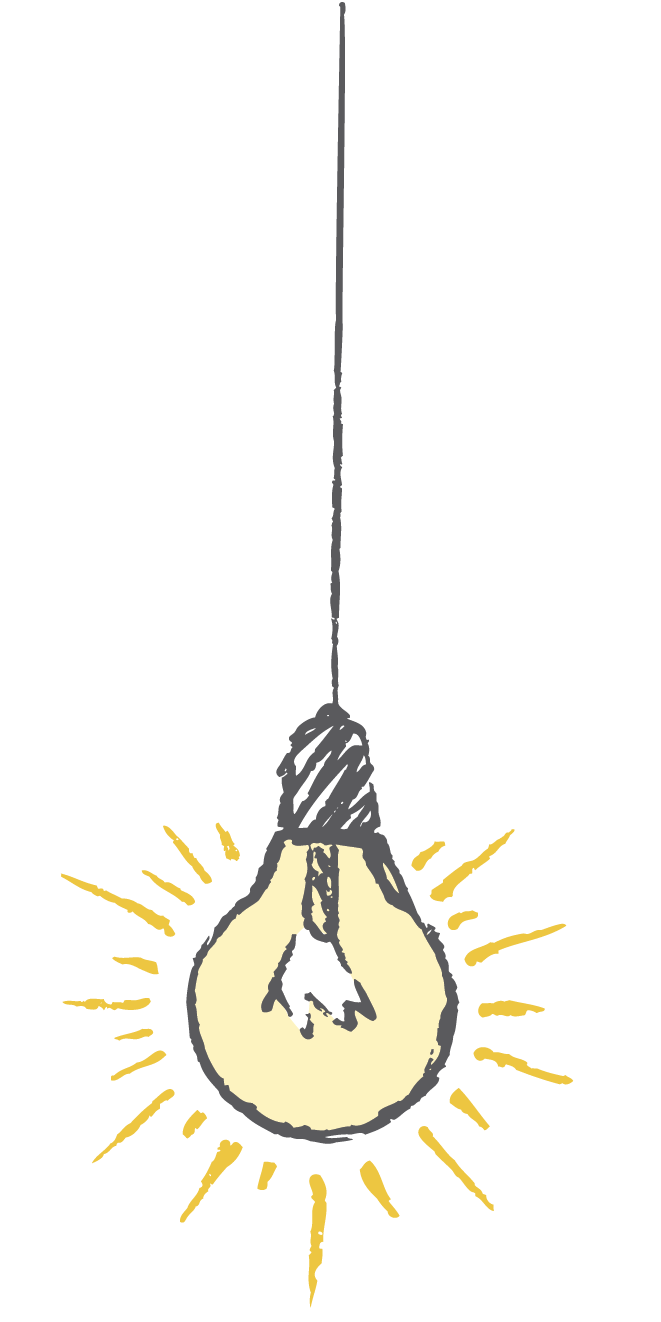
\includegraphics[width=\linewidth]{light.png}
\end{marginfigure}

\begin{abstract}
This Exercise will introduce new users to the features of the command \textbf{ietestform} that is developed by DIME Analytics. \textbf{ietestform} collects years at DIME in how to code high quality SurveyCTO questionnaires.


\bigskip\noindent \textbf{Exercise Objectives}:
\begin{enumerate}
  \item Learn how to run the command
  \item Learn what the most common tests are testing for and why
  \item Learn how to use the documentation 
\end{enumerate}
\end{abstract}

%\printclassoptions
\section{Intro and context for the exercise}

Coding a complex questionnaire is difficult, especially since it next to impossible to keep a good overview of your Excel form template once it reached several hundreds of rows of code which is the norm rather than the exception.

While it ends up being very challenging for a human eye to catch a typo in a single out of hundreds of row, that is pose no challenge to a computer once we have developed a way to express in code what is very likely a typo. One example is if we have 10 multiple choice list items, where 9 of them have the list name \textit{village} and one have the list name \textit{vilage}, and the list \textit{vilage} is not used. We can express a test like that in code, and that one example of the many test that \verb|ietestform| is developed to do on your SurveyCTO forms.

Other examples are test that no fields of type \textit{note} are required, test that no two multiple choice codes has the same label, test that non standard characters are used in field names that will later cause problem when loading it in Stata. Sometimes some of these things are intentional, so all the cases that \verb|ietestform| flag are not always errors, but a human should pay extra attention to each case flagged to see whether it is an error or not.

%\printclassoptions
\section{Part 1: Run ietestform}

	We have prepared a do-file\sidenote{see the file handson\_iestestform.do provided in the excercise material or in the code example below} for you that make sure you have |ietoolkit| and |iefielkit| installed and that you are using the most recent version of |iefieldkit|. It also uses |ieboilstart| to harmonize version and memory settings, and lastly sets up a global path file to the folder we will work in before it runs the command.
	
	After you have filled in your user name\sidenote{In \verb|"`c(username)'" == ""| replace the \verb|""| with your computers username} and your file path\sidenote{In \verb|global folder ""| replace the \verb|""| with your file path} to the folder you want to use for this exercise, you can run this do-file and then the report will be created in the folder you specified in the folder global. Once you have been able to generate the report, move to next step.


	\begin{minipage}{1.5\textwidth}
	\vspace{.5cm}
	\VerbatimInput[frame=lines, % line above and below code section
	 			   numbers=left, %Line number
	 			   label=handson\_ietestform.do, %name of code section
	 			   samepage=true, %Do not allow the code to be broken across pages
	 			   baselinestretch=0.75 %Use line space more similat to line space in code editors
	 			  ]{./handson_ietestform.do}
 	\end{minipage}


%\printclassoptions
\section{Part 2: Read the output}



%\printclassoptions
\section{Part 3: Use the documentation}

\end{document}
